%%%%%%%%%%%%%%%%%%%%%%%%%%%%%%%%
%                              %
% Luther Michaels              % 
% ECE 351-52                   %
% Lab 8                        %
% October 21, 2021             %
% Fourier Series Approximation % 
%             of a Square Wave %
%                       Prelab %
%                              %
%%%%%%%%%%%%%%%%%%%%%%%%%%%%%%%%

%%%%%%%%%%%%%%%%%%%%%%%%%%%%%%%%%%%%%%%%%%%
%%% DOCUMENT PREAMBLE %%%
\documentclass[12pt]{report}
\usepackage[english]{babel}
\usepackage{url}
\usepackage[utf8x]{inputenc}
\usepackage{amsmath}
\usepackage{graphicx}
\graphicspath{{images/}}
\usepackage{parskip}
\usepackage{fancyhdr}
\usepackage{vmargin}
\usepackage{listings}
\usepackage{hyperref}
\usepackage{xcolor}

\definecolor{codegreen}{rgb}{0,0.6,0}
\definecolor{codegray}{rgb}{0.5,0.5,0.5}
\definecolor{codeblue}{rgb}{0,0,0.95}
\definecolor{backcolour}{rgb}{0.95,0.95,0.92}

\lstdefinestyle{mystyle}{
	backgroundcolor=\color{backcolour},   
	commentstyle=\color{codegreen},
	keywordstyle=\color{codeblue},
	numberstyle=\tiny\color{codegray},
	stringstyle=\color{codegreen},
	basicstyle=\ttfamily\footnotesize,
	breakatwhitespace=false,         
	breaklines=true,                 
	captionpos=b,                    
	keepspaces=true,                 
	numbers=left,                    
	numbersep=5pt,                  
	showspaces=false,                
	showstringspaces=false,
	showtabs=false,                  
	tabsize=2
}

\lstset{style=mystyle}

\setmarginsrb{3 cm}{2.5 cm}{3 cm}{2.5 cm}{1 cm}{1.5 cm}{1 cm}{1.5 cm}

\title{8}	% Title						
\author{Luther Michaels}	% Author		
\date{October 21, 2021}   % Date

\makeatletter
\let\thetitle\@title
\let\theauthor\@author
\let\thedate\@date
\makeatother

\pagestyle{fancy}
\fancyhf{}
\rhead{\theauthor}
\lhead{\thetitle}
\cfoot{\thepage}
%%%%%%%%%%%%%%%%%%%%%%%%%%%%%%%%%%%%%%%%%%%%

\begin{document}
	
%%%%%%%%%%%%%%%%%%%%%%%%%%%%%%%%%%%%%%%%%%%%%%%%%%%%%%%%%%%%%%%%%%%%%%%%%%%%%%%%%%
%%% TITLE PAGE %%%
\begin{titlepage}
	\centering
	\vspace*{0.5 cm}
		
	\begin{center}    
		\textsc{\Large   ECE 351 - Section \#52}\\[2.0 cm]	
	\end{center}  
	\textsc{\Large Fourier Series Approximation \\ of a Square Wave (Prelab)  }\\[0.5 cm]
	\rule{\linewidth}{0.2 mm} \\[0.4 cm]
	{ \huge \bfseries \thetitle}\\
	\rule{\linewidth}{0.2 mm} \\[1.5 cm]
	\begin{minipage}{0.4\textwidth}
		\begin{flushleft} \large
		\end{flushleft}
	\end{minipage}~
	\begin{minipage}{0.4\textwidth}
		\begin{flushright} \large
			\emph{Submitted By:} \\
			Luther Michaels \break
				
			\emph{Submission Date:} \\
			October 21, 2021
		\end{flushright}
	\end{minipage}\\[2 cm]
\end{titlepage}
	
%%%%%%%%%%%%%%%%%%%%%%%%%%%%%%%%%%%%%%%%%%%%%%%%%%%%%%%%%%%%%%%%%%%%%%%%%%%%%%%%%%
%%% LAB PRELAB %%%
\renewcommand{\thesection}{\arabic{section}}
	
\section{Setup}
	
\begin{center}
		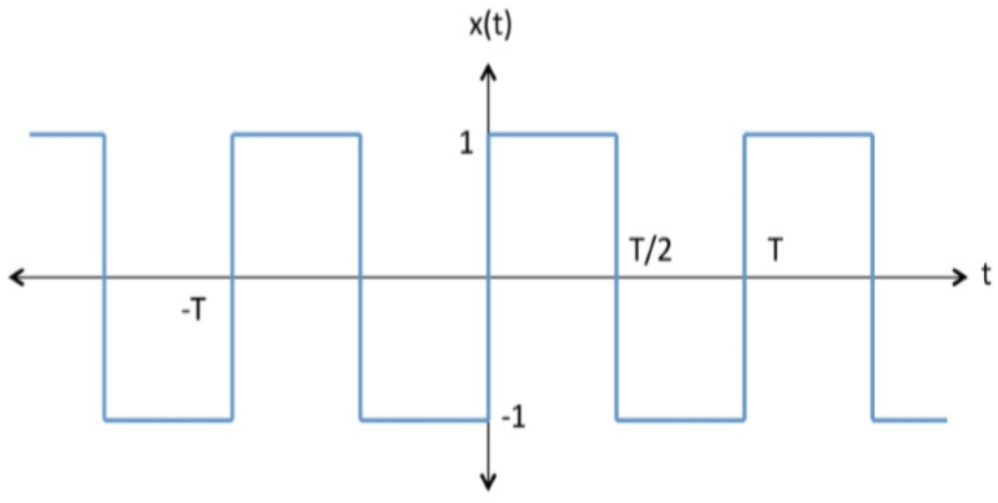
\includegraphics[scale = 0.6]{Lab 8 - Plots/Prelab.png}\\[1.0 cm]
\end{center}
\begin{equation}
	x(t) = \frac{1}{2}a_0 + \sum_{k=1}^{\infty}a_kcos(kw_0t) + b_ksin(kw_0t)
	\end{equation}
Where, \\
\begin{equation}
	a_k = \frac{2}{T}\int_{0}^{T}x(t)cos(kw_0t)dt
\end{equation}
\begin{equation}
	b_k = \frac{2}{T}\int_{0}^{T}x(t)sin(kw_0t)dt
\end{equation}
\begin{equation}
	w_0 = \frac{2\pi}{T}
\end{equation}
	
\section{Derive $ a_k $, $ b_k $, and $ x(t) $}
	
\begin{equation*}
	x_0(t) = p_{\frac{T}{2}}(t - \frac{T}{4}) - p_{\frac{T}{2}}(t - \frac{3T}{4})
\end{equation*}
\begin{align*}
	a_k &= \frac{2}{T}\int_{0}^{T}x(t)cos(\frac{2\pi kt}{T})dt \\
	&= \frac{2}{T}\int_{0}^{\frac{T}{2}}(1)cos(\frac{2\pi kt}{T})dt + \frac{2}{T}\int_{\frac{T}{2}}^{T}(-1)cos(\frac{2\pi kt}{T})dt \\
	&= \frac{2}{T}\int_{0}^{\frac{T}{2}}cos(\frac{2\pi kt}{T})dt - \frac{2}{T}\int_{\frac{T}{2}}^{T}cos(\frac{2\pi kt}{T})dt \\
	&= \frac{1}{\pi k}[sin(2\pi kt)]|_0^{\frac{T}{2}} - \frac{1}{\pi k}[sin(2\pi kt)]|_{\frac{T}{2}}^{T} \\
	&= \frac{1}{\pi k}sin(\pi kT) - \frac{1}{\pi k}[sin(2\pi kT) - sin(\pi kT)] \\
	&= \frac{1}{\pi k}[2sin(\pi kT) - sin(2\pi kT)]
\end{align*}
\begin{align*}
	b_k &= \frac{2}{T}\int_{0}^{T}x(t)sin(\frac{2\pi kt}{T})dt \\
	&= \frac{2}{T}\int_{0}^{\frac{T}{2}}(1)sin(\frac{2\pi kt}{T})dt + \frac{2}{T}\int_{\frac{T}{2}}^{T}(-1)sin(\frac{2\pi kt}{T})dt \\
	&= \frac{2}{T}\int_{0}^{\frac{T}{2}}sin(\frac{2\pi kt}{T})dt - \frac{2}{T}\int_{\frac{T}{2}}^{T}sin(\frac{2\pi kt}{T})dt \\
	&= -\frac{1}{\pi k}[cos(2\pi kt)]|_0^{\frac{T}{2}} + \frac{1}{\pi k}[cos(2\pi kt)]|_{\frac{T}{2}}^{T} \\
	&= \frac{1}{\pi k}[1 - cos(\pi kT)] + \frac{1}{\pi k}[cos(2\pi kT)) - cos(\pi kT)] \\
	&= \frac{1}{\pi k}[1 + cos(2\pi kT) - 2cos(\pi kT)]
\end{align*}
\begin{equation*}
	a_0 = 0
\end{equation*}
\begin{align*}
	x(t) = \sum_{k=1}^{\infty}\frac{1}{\pi k}[2sin(\pi kT) - sin(2\pi kT)]cos(\frac{2\pi kt}{T}) + \frac{1}{\pi k}[1 + cos(2\pi kT) - 2cos(\pi kT)]sin(\frac{2\pi kt}{T})
\end{align*}
	
\end{document}

% Lab Report based on template created by Roza Aceska.